\chapter{System Design}

\section{Introduction}

This chapter presents the architectural design of Reel Forge AI, including system architecture, database design, API specifications, and user interface design. The design emphasizes modularity, scalability, and maintainability.

\section{System Architecture}

\subsection{Overall Architecture}

Reel Forge AI follows a three-tier architecture:

\begin{enumerate}
    \item \textbf{Presentation Layer:} React-based single-page application
    \item \textbf{Application Layer:} Node.js/Express REST API server
    \item \textbf{Data Layer:} PostgreSQL relational database
\end{enumerate}

\begin{figure}[H]
\centering
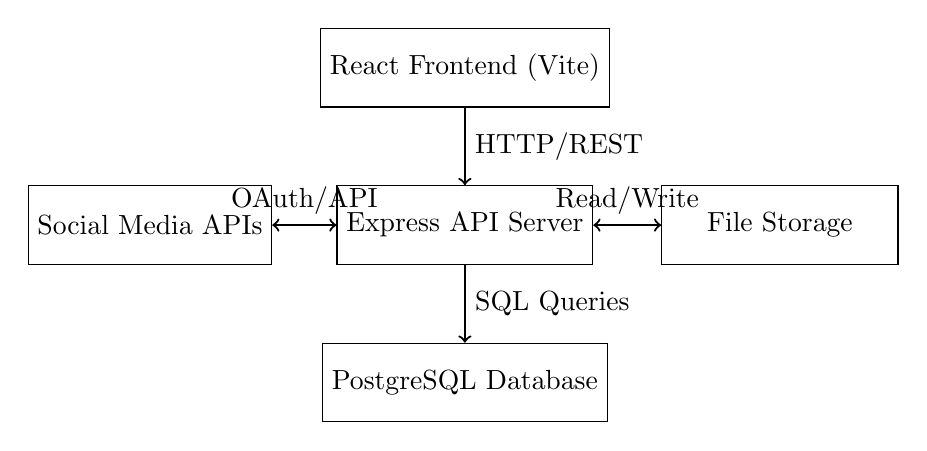
\begin{tikzpicture}[node distance=2cm]
    % Nodes
    \node (client) [rectangle, draw, minimum width=3cm, minimum height=1cm] {React Frontend (Vite)};
    \node (api) [rectangle, draw, minimum width=3cm, minimum height=1cm, below of=client] {Express API Server};
    \node (db) [rectangle, draw, minimum width=3cm, minimum height=1cm, below of=api] {PostgreSQL Database};
    \node (storage) [rectangle, draw, minimum width=3cm, minimum height=1cm, right of=api, xshift=2cm] {File Storage};
    \node (social) [rectangle, draw, minimum width=3cm, minimum height=1cm, left of=api, xshift=-2cm] {Social Media APIs};
    
    % Arrows
    \draw[->, thick] (client) -- node[right] {HTTP/REST} (api);
    \draw[->, thick] (api) -- node[right] {SQL Queries} (db);
    \draw[<->, thick] (api) -- node[above] {Read/Write} (storage);
    \draw[<->, thick] (api) -- node[above] {OAuth/API} (social);
\end{tikzpicture}
\caption{High-Level System Architecture}
\end{figure}

\subsection{Component Architecture}

The application is organized into modular components:

\begin{description}
    \item[Authentication Module:] User registration, login, session management
    \item[Video Processing Module:] Upload handling, transcript generation, clip cutting
    \item[Social Integration Module:] OAuth flows, API integrations for YouTube/Facebook/Instagram
    \item[Project Management Module:] CRUD operations for projects and clips
    \item[Storage Module:] File upload, storage, retrieval, and cleanup
    \item[Batch Processing Module:] Asynchronous job queue for heavy processing tasks
\end{description}

\subsection{Technology Stack}

\begin{table}[H]
\centering
\caption{Technology Stack Summary}
\begin{tabular}{@{}lll@{}}
\toprule
\textbf{Layer} & \textbf{Technology} & \textbf{Purpose} \\
\midrule
Frontend & React 18 & UI component library \\
 & TypeScript & Type-safe development \\
 & Vite & Build tool and dev server \\
 & TailwindCSS & Utility-first styling \\
 & shadcn/ui & UI component library \\
 & TanStack Query & Data fetching and caching \\
\midrule
Backend & Node.js & JavaScript runtime \\
 & Express & Web application framework \\
 & TypeScript & Type-safe development \\
 & Drizzle ORM & Database abstraction \\
 & express-session & Session management \\
\midrule
Database & PostgreSQL & Relational database \\
\midrule
Processing & FFmpeg & Video manipulation \\
 & OpenAI API & Speech-to-text \\
\midrule
Integration & googleapis & YouTube API client \\
 & axios & HTTP client \\
 & form-data & Multipart form handling \\
\midrule
Deployment & Docker & Containerization \\
 & Nginx & Reverse proxy \\
\bottomrule
\end{tabular}
\end{table}

\section{Database Design}

\subsection{Entity-Relationship Diagram}

\begin{figure}[H]
\centering
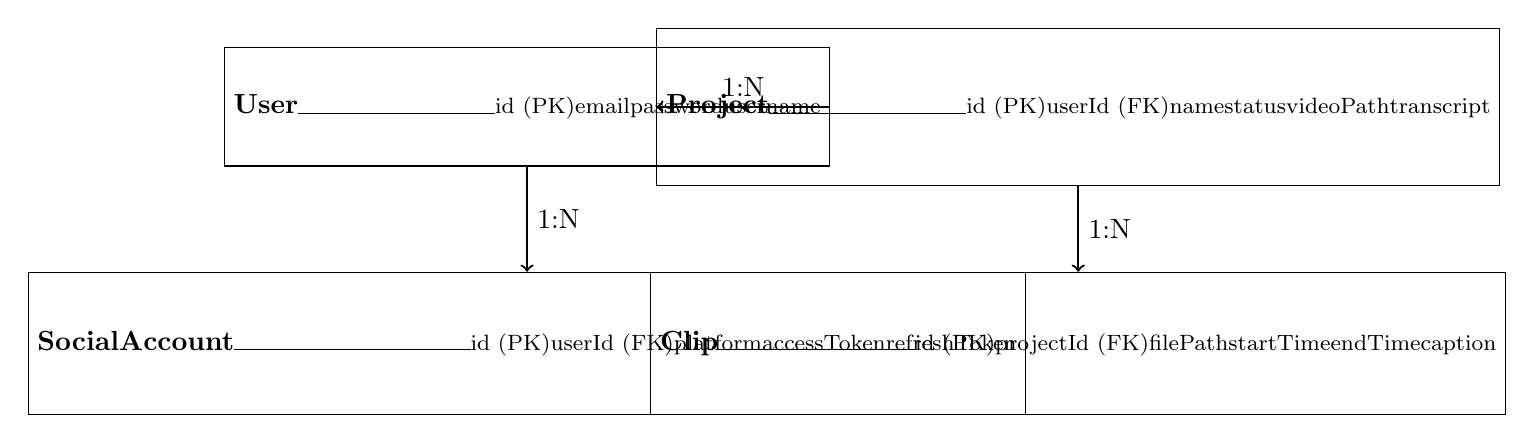
\begin{tikzpicture}[node distance=3cm]
    % Entities
    \node (user) [rectangle, draw, minimum width=2.5cm, minimum height=1.5cm] {
        \textbf{User}\\
        \rule{2.5cm}{0.4pt}\\
        \footnotesize id (PK)\\
        email\\
        password\\
        username
    };
    
    \node (project) [rectangle, draw, minimum width=2.5cm, minimum height=2cm, right of=user, xshift=4cm] {
        \textbf{Project}\\
        \rule{2.5cm}{0.4pt}\\
        \footnotesize id (PK)\\
        userId (FK)\\
        name\\
        status\\
        videoPath\\
        transcript
    };
    
    \node (clip) [rectangle, draw, minimum width=2.5cm, minimum height=1.8cm, below of=project] {
        \textbf{Clip}\\
        \rule{2.5cm}{0.4pt}\\
        \footnotesize id (PK)\\
        projectId (FK)\\
        filePath\\
        startTime\\
        endTime\\
        caption
    };
    
    \node (social) [rectangle, draw, minimum width=3cm, minimum height=1.8cm, below of=user] {
        \textbf{SocialAccount}\\
        \rule{3cm}{0.4pt}\\
        \footnotesize id (PK)\\
        userId (FK)\\
        platform\\
        accessToken\\
        refreshToken
    };
    
    % Relationships
    \draw[->, thick] (user) -- node[above] {1:N} (project);
    \draw[->, thick] (project) -- node[right] {1:N} (clip);
    \draw[->, thick] (user) -- node[right] {1:N} (social);
\end{tikzpicture}
\caption{Entity-Relationship Diagram}
\end{figure}

\subsection{Database Schema}

\subsubsection{User Table}

\begin{lstlisting}[language=SQL, caption=User Table Schema]
CREATE TABLE users (
    id SERIAL PRIMARY KEY,
    email VARCHAR(255) UNIQUE NOT NULL,
    password VARCHAR(255) NOT NULL,
    username VARCHAR(255),
    created_at TIMESTAMP DEFAULT CURRENT_TIMESTAMP,
    updated_at TIMESTAMP DEFAULT CURRENT_TIMESTAMP
);

CREATE INDEX idx_users_email ON users(email);
\end{lstlisting}

\subsubsection{Project Table}

\begin{lstlisting}[language=SQL, caption=Project Table Schema]
CREATE TABLE projects (
    id UUID PRIMARY KEY DEFAULT gen_random_uuid(),
    user_id INTEGER REFERENCES users(id) ON DELETE CASCADE,
    name VARCHAR(255) NOT NULL,
    status VARCHAR(50) DEFAULT 'processing',
    progress INTEGER DEFAULT 0,
    current_step TEXT,
    video_path TEXT,
    transcript TEXT,
    created_at TIMESTAMP DEFAULT CURRENT_TIMESTAMP,
    updated_at TIMESTAMP DEFAULT CURRENT_TIMESTAMP
);

CREATE INDEX idx_projects_user_id ON projects(user_id);
CREATE INDEX idx_projects_status ON projects(status);
\end{lstlisting}

\subsubsection{Clip Table}

\begin{lstlisting}[language=SQL, caption=Clip Table Schema]
CREATE TABLE clips (
    id SERIAL PRIMARY KEY,
    project_id UUID REFERENCES projects(id) ON DELETE CASCADE,
    file_path TEXT NOT NULL,
    title VARCHAR(255),
    caption TEXT,
    start_time REAL,
    end_time REAL,
    duration REAL,
    thumbnail_path TEXT,
    created_at TIMESTAMP DEFAULT CURRENT_TIMESTAMP
);

CREATE INDEX idx_clips_project_id ON clips(project_id);
\end{lstlisting}

\subsubsection{Social Media Accounts Table}

\begin{lstlisting}[language=SQL, caption=Social Media Accounts Table Schema]
CREATE TABLE social_media_accounts (
    id SERIAL PRIMARY KEY,
    user_id INTEGER REFERENCES users(id) ON DELETE CASCADE,
    platform VARCHAR(50) NOT NULL,
    access_token TEXT NOT NULL,
    refresh_token TEXT,
    token_expires_at TIMESTAMP,
    platform_user_id VARCHAR(255),
    platform_username VARCHAR(255),
    created_at TIMESTAMP DEFAULT CURRENT_TIMESTAMP,
    updated_at TIMESTAMP DEFAULT CURRENT_TIMESTAMP,
    UNIQUE(user_id, platform)
);

CREATE INDEX idx_social_accounts_user_platform 
    ON social_media_accounts(user_id, platform);
\end{lstlisting}

\section{API Design}

\subsection{RESTful API Structure}

The API follows REST principles with resource-oriented URLs:

\begin{table}[H]
\centering
\caption{API Endpoint Summary}
\begin{tabular}{@{}llp{6cm}@{}}
\toprule
\textbf{Method} & \textbf{Endpoint} & \textbf{Description} \\
\midrule
POST & /api/register & Create new user account \\
POST & /api/login & Authenticate user \\
POST & /api/logout & End user session \\
GET & /api/user & Get current user info \\
\midrule
POST & /api/projects & Create new project \\
GET & /api/projects & List all user projects \\
GET & /api/projects/:id & Get specific project \\
DELETE & /api/projects/:id & Delete project \\
\midrule
POST & /api/upload & Upload video file \\
POST & /api/social/upload & Upload to social platform \\
\midrule
GET & /api/social/youtube/auth & Initiate YouTube OAuth \\
GET & /api/social/youtube/callback & YouTube OAuth callback \\
GET & /api/social/facebook/auth & Initiate Facebook OAuth \\
GET & /api/social/facebook/callback & Facebook OAuth callback \\
DELETE & /api/social/:platform & Disconnect platform \\
\bottomrule
\end{tabular}
\end{table}

\subsection{Request/Response Formats}

All API endpoints use JSON for request and response bodies.

\subsubsection{Authentication Example}

\begin{lstlisting}[language=JavaScript, caption=Login Request/Response]
// Request
POST /api/login
Content-Type: application/json

{
  "email": "user@example.com",
  "password": "securepassword123"
}

// Response (Success)
200 OK
{
  "ok": true,
  "user": {
    "id": 1,
    "email": "user@example.com",
    "username": "John Doe"
  }
}

// Response (Error)
401 Unauthorized
{
  "ok": false,
  "message": "Invalid credentials"
}
\end{lstlisting}

\subsubsection{Project Creation Example}

\begin{lstlisting}[language=JavaScript, caption=Create Project Request/Response]
// Request
POST /api/projects
Content-Type: multipart/form-data

{
  "name": "My Video Project",
  "video": <file upload>
}

// Response
201 Created
{
  "ok": true,
  "project": {
    "id": "550e8400-e29b-41d4-a716-446655440000",
    "name": "My Video Project",
    "status": "processing",
    "progress": 0,
    "createdAt": "2026-03-01T10:00:00Z"
  }
}
\end{lstlisting}

\section{Video Processing Pipeline}

\subsection{Processing Workflow}

\begin{figure}[H]
\centering
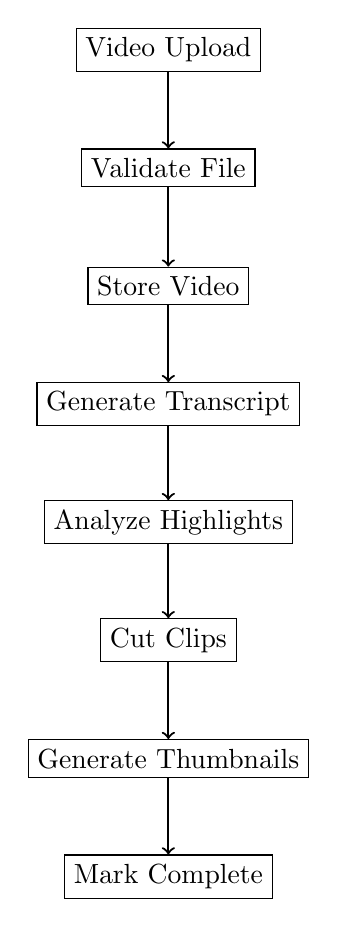
\begin{tikzpicture}[node distance=1.5cm, auto]
    \node (upload) [rectangle, draw] {Video Upload};
    \node (validate) [rectangle, draw, below of=upload] {Validate File};
    \node (store) [rectangle, draw, below of=validate] {Store Video};
    \node (transcript) [rectangle, draw, below of=store] {Generate Transcript};
    \node (analyze) [rectangle, draw, below of=transcript] {Analyze Highlights};
    \node (cut) [rectangle, draw, below of=analyze] {Cut Clips};
    \node (thumbnail) [rectangle, draw, below of=cut] {Generate Thumbnails};
    \node (complete) [rectangle, draw, below of=thumbnail] {Mark Complete};
    
    \draw[->, thick] (upload) -- (validate);
    \draw[->, thick] (validate) -- (store);
    \draw[->, thick] (store) -- (transcript);
    \draw[->, thick] (transcript) -- (analyze);
    \draw[->, thick] (analyze) -- (cut);
    \draw[->, thick] (cut) -- (thumbnail);
    \draw[->, thick] (thumbnail) -- (complete);
\end{tikzpicture}
\caption{Video Processing Pipeline}
\end{figure}

\subsection{AI Analysis Algorithm}

\begin{lstlisting}[language=JavaScript, caption=Highlight Detection Pseudocode]
function detectHighlights(transcript) {
  const sentences = splitIntoSentences(transcript);
  const scored = [];
  
  for (let i = 0; i < sentences.length; i++) {
    let score = 0;
    
    // Keyword scoring
    score += countEngagementKeywords(sentences[i]);
    
    // Context window analysis
    const context = getContextWindow(sentences, i, 3);
    score += analyzeContextCoherence(context);
    
    // Pacing analysis
    score += analyzeSentencePacing(sentences[i]);
    
    scored.push({ sentence: sentences[i], score, index: i });
  }
  
  // Select top N scoring segments
  const highlights = scored
    .sort((a, b) => b.score - a.score)
    .slice(0, 3);
  
  return highlights.map(h => ({
    start: h.index * avgSentenceDuration,
    end: (h.index + 1) * avgSentenceDuration,
    text: h.sentence
  }));
}
\end{lstlisting}

\section{Security Design}

\subsection{Authentication Flow}

\begin{enumerate}
    \item User submits credentials via HTTPS
    \item Server validates credentials against hashed password
    \item Server creates encrypted session token
    \item Session stored in secure, HTTP-only cookie
    \item Subsequent requests include session cookie
    \item Server validates session on each request
\end{enumerate}

\subsection{OAuth 2.0 Flow}

\begin{enumerate}
    \item User initiates OAuth connection
    \item System generates state token for CSRF protection
    \item User redirected to platform authorization page
    \item User grants permissions
    \item Platform redirects with authorization code
    \item System exchanges code for access token
    \item Access token encrypted and stored in database
    \item Refresh token stored for token renewal
\end{enumerate}

\subsection{Data Protection Measures}

\begin{itemize}
    \item Password hashing using bcrypt (cost factor: 10)
    \item OAuth tokens encrypted using AES-256
    \item Session cookies with HTTP-only and Secure flags
    \item CSRF tokens for state-changing operations
    \item Input sanitization and validation
    \item SQL injection prevention via parameterized queries
    \item Rate limiting on authentication endpoints
\end{itemize}

\section{User Interface Design}

\subsection{Design Principles}

\begin{enumerate}
    \item \textbf{Simplicity:} Minimal steps to accomplish tasks
    \item \textbf{Clarity:} Clear visual hierarchy and feedback
    \item \textbf{Consistency:} Uniform design patterns throughout
    \item \textbf{Responsiveness:} Adaptive layout for all devices
    \item \textbf{Accessibility:} WCAG 2.1 AA compliance
\end{enumerate}

\subsection{Page Structure}

\begin{description}
    \item[Landing Page:] Hero section, features overview, call-to-action
    \item[Authentication Pages:] Login, registration, password reset forms
    \item[Dashboard:] Project overview, statistics, quick actions
    \item[Create Page:] Video upload interface with drag-and-drop
    \item[Processing Page:] Real-time progress indicators and status updates
    \item[Library Page:] Grid view of processed clips with download/share options
    \item[Settings Page:] Social media connections, profile management
\end{description}

\subsection{Component Design}

Key UI components include:
\begin{itemize}
    \item Sidebar navigation with responsive collapse
    \item Project cards with status badges
    \item Video player with controls
    \item Social media platform buttons with connection status
    \item Progress indicators (linear and circular)
    \item Modal dialogs for confirmations
    \item Toast notifications for user feedback
    \item Theme toggle (dark/light mode)
\end{itemize}

\section{Error Handling Strategy}

\subsection{Error Categories}

\begin{enumerate}
    \item \textbf{Client Errors (400s):} Invalid input, authentication failures
    \item \textbf{Server Errors (500s):} Processing failures, database errors
    \item \textbf{External Errors:} Third-party API failures, network issues
\end{enumerate}

\subsection{Error Response Format}

\begin{lstlisting}[language=JavaScript, caption=Standard Error Response]
{
  "ok": false,
  "message": "User-friendly error message",
  "error": {
    "code": "ERROR_CODE",
    "details": "Technical error details for debugging"
  }
}
\end{lstlisting}

\subsection{Graceful Degradation}

\begin{itemize}
    \item Fallback mechanisms for failed AI processing
    \item Queue retry logic for transient failures
    \item Default values for missing optional data
    \item User-friendly error messages with recovery suggestions
    \item Automatic cleanup of incomplete operations
\end{itemize}

\section{Performance Optimization}

\subsection{Frontend Optimization}

\begin{itemize}
    \item Code splitting and lazy loading
    \item Image and video optimization
    \item React Query caching for API responses
    \item Debouncing for search and input operations
    \item Virtual scrolling for large lists
\end{itemize}

\subsection{Backend Optimization}

\begin{itemize}
    \item Database connection pooling
    \item Query optimization with proper indexing
    \item Caching frequently accessed data
    \item Async/await for non-blocking operations
    \item Stream processing for large files
\end{itemize}

\section{Summary}

This chapter has presented a comprehensive system design for Reel Forge AI, covering architecture,database schema, API specifications, security measures, and user interface design. The modular architecture ensures maintainability and scalability, while security measures protect user data and credentials. The design forms a solid foundation for implementation discussed in the next chapter.
